\documentclass[useAMS,usenatbib]{mn2e}
%\documentclass[a4paper,15pt]{article}
%\documentclass[a4paper,10pt]{article}
%\usepackage{aas_macros}
\usepackage{myaasmacros}
\usepackage{graphicx}
\usepackage{color}
\usepackage{amsmath}
\usepackage{hyperref}
%\usepackage{amssym}
%\usepackage{times}
%\usepackage{arial}
%\bibliographystyle{abbrv}
%\bibliographystyle{plain}
%\bibliographystyle{apalike}
%\bibliographystyle{mn2e}
%% mn2e style
% \documentclass[useAMS,usenatbib]{mn2e}
% \usepackage{aas_macros}
% \usepackage[dvips]{graphicx}
% \usepackage{amssymb,amsmath}
% \thispagestyle{headings}
% \usepackage{xcolor}
% \usepackage{graphicx}
% \bibliographystyle{mn2e}%abbrv,plain,apalike

% article/research plan style
\documentclass[a4paper]{article}
\usepackage[T1]{fontenc}
\usepackage[latin1]{inputenc}
\usepackage{natbib}
\usepackage[pdftex]{graphicx}
\usepackage{color}
\usepackage{amssymb}
\usepackage[sumlimits, namelimits, reqno]{amsmath}
\usepackage{aas_macros}
\bibliographystyle{apalike}
% available bibliography styles: apalike %abbrv, plain, natbib, dcu (use harvard as well)

% \usepackage{textcomp}
% \usepackage{scrpage2}
% \usepackage{mathpazo}
% \usepackage[scaled=.9]{helvet}

\newcommand\bcite[1]{(\citeauthor{#1} \citeyear{#1})}
\newcommand{\changefont}[3]{
\fontfamily{#1} \fontseries{#2} \fontshape{#3} \selectfont}
\newcommand{\TODO}[1]{\textsc{\textbf{\textcolor{red}{(TODO: #1)}}}}



% Some definitions for the priors:
\def\gprior{{\tt gprior}}
\def\cprior{{\tt cprior}}
\def\bprior{{\tt bprior}}
\def\lbprior{{\tt lbprior}}

%Some definitions for rhodm etc:
\def\vztwo{\overline{v_z^2}}
\def\vztwoi{\overline{v_{z,i}^2}}
\def\rhodisc{\rho_\mathrm{disc}(z)}
\def\rhodmext{\rho_\mathrm{dm,ext}}
\def\rhodm{\rho_\mathrm{dm}}
\def\rhoeff{\rho_\mathrm{dm}^\mathrm{eff}}
\def\nuobs{\nu_\mathrm{obs}(z)}

\def\ltsima{$\; \buildrel < \over \sim \;$}
\def\simlt{\lower.5ex\hbox{\ltsima}}
\def\gtsima{$\; \buildrel > \over \sim \;$}
\def\simgt{\lower.5ex\hbox{\gtsima}}
\def\siglos{\sigma_{\text{LOS}}}
\def\siglosi{\sigma_{\text{LOS},i}}
\def\kaplos{\kappa_{\text{LOS}}}

% units for inside math environments
\def\keV{\mathrm{keV}}
\def\MeV{\mathrm{MeV}}
\def\GeV{\mathrm{GeV}}
\def\Msun{M_{\odot}}
\def\pc{\mathrm{pc}}
\def\kpc{\mathrm{kpc}}
\def\Mpc{\mathrm{Mpc}}
\def\K{\mathrm{K}}

\title[Generations in Bounded Confidence]{Generations in the Bounded Confidence Model}
\author[P. Steger]{P. Steger$^{1}$\thanks{E-mail: psteger@phys.ethz.ch},\\
 $^{1}$Department of Physics, ETH Z\"urich, CH-8093 Z\"urich,
 Switzerland
}


\begin{document}

\date{May 2014}
\label{firstpage}
\maketitle

\begin{abstract}
    I investigate the evolution and stability of an
    agent based model for opinions in a group of agents with a
    finite lifetime.

    I answer the following questions: What conditions must be fulfilled to
    enable a significant change in the consensus of an opinion group?
    What is the typical timescale before such a change occurs?
\end{abstract}

\begin{keywords}
 Bounded Confidence Model: Opinion Groups, Evolution --
 Methods: Numerical
\end{keywords}


%TODO search for literature
%TODO arxiv Lorenz bounded confidence models, search for perturbations / noise

\section{Motivation}
\label{sec:motivation}
The bounded confidence model describes the way an ensemble of agents
converges on a common opinion, or several final opinions.

An effect that cannot be described with this model is long-time change
of opinions, as is e.g. seen in human societies over several
generations. A prominent example would be the support for governmental control
in the U.S., as e.g. studied by (Coggins+ 2013)\footnote{under review,
\url{www.unc.edu/~mlatkins/docs/OpinionChange_CSAB.pdf}}.

I want to model the evolution of opinions with time, when new agents
without bias appear in the system, by adding one additional internal
parameter for an agent: its age.

I propose that as old agents disappear and are replaced by young,
unbiased agents, noise is introduced and a shift in the overall
opinion occurs. The conditions allowing the opinion of a group to
change significantly are investigated.


\section{Model and Rules}
\label{sec:model}

We model agents $i\in[1,N]$ with two internal parameters: an opinion
$o_i$ and an age $a_i$.

Initial conditions are set such that the opinions are uniformly
distributed. The creation times of the agents are also unfiormly
distributed over the span $[-a_{\rm max},0]$, where $a_{\rm max}$ is the maximum lifetime
of an agent. 

We introduce a distance $d$ between two agents measured with a metric

\begin{equation}
    d(o_i,o_j,x_i, x_j) =
    \begin{cases}
        |o_i-o_j|/\varepsilon,&{\rm opinion space},\\
        |a_i-a_j|/\varepsilon,&{\rm temporal space},
    \end{cases}
\end{equation}

with opinions $o_i$, age $a_i$, and fudge
parameters $\alpha, \beta$. They determine which part of the social distance is
considered: Only difference in opinions, only difference in age, or
both. For sake of simplicity, I restrict myself to distance in the
opinion space, $\alpha=1, \beta=0$. 

In each timestep, two random
agents meet. They interact with interaction strength

\begin{equation}
    \Sigma = \frac{1}{1+\exp\left(\frac{d-\varepsilon}{s\varepsilon}\right)}
\end{equation}

such that for a distance $d$ smaller than scale $\varepsilon$ the
interaction reaches maximum strength 1, and falls off to 0 at
$\varepsilon$ over a distance $s$.

The interaction is based on the bounded confidence model

\begin{eqnarray}
    o_i(t+1) &=& o_i(t)+\zeta\cdot(o_j(t)-o_i(t))\\
    o_j(t+1) &=& o_j(t)+\zeta\cdot(o_i(t)-o_j(t))
\end{eqnarray}

For $\zeta=0.5$, the agents adjust their opinion to the average of both
opinions.


I define groups to be sets of agents with a common opinion, such that

\begin{enumerate}
    \item they contain at least two members or 10 percent of the fraction
    that is theoretically expected to be contained in the maximal
    influence region $1/(2\varepsilon)$;
    \item their agents are closer to each other than to any
    non-member. This is ensured by a hierarchical clustering algorithm
    with cut at $\varepsilon/2$. A classical $k$-means algorithm does
    not work, as one needs a-priori knowledge about the number of groups
    one wants to find. This number is not constant in the dynamic
    evolution we are looking at.
\end{enumerate}

\section{Analytic Treatment}
\label{sec:analytic}

\subsection{Decay of prevalent consensus}
Let us first determine the decay of a prevalent consensus. We start
with the following setup: All $N$ agents of a population have converged on
a common consensus $c$, and thus their opinion distribution is given
by

\begin{equation}
    \label{eq:opiniondistribution_consensus}
    D_{\rm old}(o)=\delta(o-c)
\end{equation}

as a function of opinion $o$, consensus opinion $c$, and delta
function $\delta$, such that the distribution is normalized to

\begin{equation}
    \label{eq:opiniondistribution_consensus_normalization}
    \int_{-\infty}^{\infty} D_{\rm old}(o) do = 1
\end{equation}

I will assume a uniform age distribution,

\begin{equation}
    \label{eq:agedistribution}
    A(a) = \frac{1}{a_{\rm max}-0} = \frac{1}{a_{\rm max}}
\end{equation}

with age $0<a<a_{\rm max}$ and normalization

\begin{equation}
    \label{eq:agedistribution_normalization}
    \tilde{A} = \int_0^{a_{\rm max}} A(a) da = \frac{1}{a_{\rm max}} \cdot (a_{\rm max}-0) = 1
\end{equation}

Now if time evolves, agents with finite lifetime $a_{\rm max}$ start
to disappear, giving a total number of ``dead'' agents

\begin{equation}
    \tilde{\Delta}(t) = \int_{a_{\rm max}}^{a_{\rm max}} = \frac{t}{a_{\rm max}}
\end{equation}

and a remaining fraction

\begin{equation}
    R(t) = \frac{\tilde{A}-\tilde{\Delta}(t)}{\tilde{A}} = 1-t/a_{\rm max}
\end{equation}

To keep things simple, I assume this subtracted fraction to be replaced by newly
created agents. These agents do not have a preset opinion, and thus
sample uniformly from the available opinion space. 

When new agents are randomly introduced and start to interact with an
opinion group, the consensus value will be corrected in the direction
of the new agents. I want to determine the timespan required for the
consensus to evolve significantly from its initial value. I define
this to be the smallest $\Delta T$ for which

\begin{equation}
    |o(T + \Delta T) - o(T)| \geq \text{std}(o(T+\Delta T))
\end{equation}

with the standard deviation $\text{std}(o(T+\Delta T))$ of all opinions inside
the group. The std is not chosen from the first group, as this
generally features a high spread in opinions and would never get
changed above that level.

To first order, the summed distribution of (remaining agents with fixed opinion)+(new
agents with random opinions in $[0,1]$) will 
feel significant influence from the new agents as soon as their
integrated opinion is of order of the consensus integral, and thus
after half the lifetime, $T=a_{\rm max}/2$. This neglects any temporal
change, which we will include in the next part.

\subsection{Steady State}

Further analytic treatment can be performed for the case of steady state. An
opinion group with $N_i(T)$ agents at time $T$ has a mean
opinion $O_i(T)$ which evolves according to Brownian motion, if new agents
with opinion $o_i$ appear inside its region of attraction $O_i(T)-\varepsilon \leq o_i
\leq O_i(T)+\varepsilon$. In steady state, it is expected that the
number of new agents corresponds to the number of removed agents. In
this case, a random walk is initiated with mean
steps of size $\varepsilon \zeta /(2 N_i)$. This gives an expected distance
covered by diffusion after $\Delta T$ steps of

\begin{equation}
    E(|O_i(T+\Delta T)-O_i(T)|) = \sqrt{\frac{2\Delta T}{\pi}\frac{\varepsilon \zeta}{2 N_i}}
\end{equation}

I assumed that $N_i\approx \text{const}$, which is not necessarily the
case as agents die, but a reasonable approximation for steady state.

I expect that as soon as this random walker in 1D evolves a distance
$\varepsilon/2$ away from its initial state, its agents begin to
interact with the adjacent group, and merge over a characteristic timescale of
$T_p = (N_i(T)/N_{\rm tot})\cdot N_{\rm it. per timestep}\cdot \zeta$. In physics, this would correspond to
a phase transition, in the style of droplet coagulation. The timescale from the first detection of a
consensus group up to a significant change in opinion can thus be
determined from

\begin{equation}
    \varepsilon/2 = E(|O_i(T+\Delta T)-O_i(T)|) =  \sqrt{\frac{2\Delta T}{\pi}\frac{\varepsilon}{2 N_i}},
\end{equation}

\begin{equation}
    \Delta T \approx \frac{\pi}{4}\frac{N_i\varepsilon}{\zeta} + T_p
\end{equation}

For a fiducial model with $\varepsilon=0.25$, $\zeta=0.1$, $N_i\approx 50\cdot
2\varepsilon = 25$ this gives a $\Delta T=40+5=45$, where 40 timesteps
are needed for group evolution, and 5 timesteps are
needed for merging.

\section{Simulation}
\label{sec:sim}

\subsection{Parameter Sweep}
\label{sec:parameter_sweep}

Independent parameters are

\begin{enumerate}
    \item the scale of the interaction bracket, $\varepsilon+s$. This
    determines the region of influence and the number of
    contemporary opinion groups. The region sampled is $[0.1, 0.2,
    0.3, 0.4, 0.5]$. From the classical bounded confidence model, we
    know that $\text{floor}(1/2\varepsilon)$ is the expected number of
    separate opinion groups.

    For values $\varepsilon<0.1$, we need a very high
    number of agents to track all possible groups. That comes from the
    fact that each groups is defined to contain at least 2
    agents. For values $\varepsilon>0.5$, we get the same result as
    for $\varepsilon=0.4$, namely that a central group forms onto which
    all agents converge.
    \item the noise introduced by replacing agents. If, as done in our
    first setup, agents die and are replaced by agents with a
    uniformly distributed opinion, this corresponds to nudgeing a
    randomly selected fraction of opinions around in the box. The
    introduced noise is given by

    \begin{equation}
        \text{Noise}=\frac{\text{number replaced agents}}{\text{number
            all
            agents}} = \frac{1}{a_\text{max}}
    \end{equation}

    We sweep the range $a_\text{max}=[20, 40, 60, 80, 100]$ for
    simulations up to a maximum time of 300. This range is motivated by
    human societies, and tracks several evolution tracks.

\end{enumerate}


\subsection{Fiducial model}

I use a fiducial simulation of the evolution of the opinions for a
population of $50$ agents to illustrate the process. The agents have a maximum
age of $40$, the simulation is run for 300 timesteps. The interaction is characterized by
$\varepsilon=0.25$, $\zeta=0.1$, and 100 interactions per timestep. In
figure \ref{fig:fiducial} one can see the formation and classification
of opinion groups. The figure on the right shows the distribution of observed timespans $\Delta T$.

As soon as the initial groups have formed, there is a timeline
associated with that group. It is only seldomly observed that a group
disappears. There is no occurence of a split into two
groups forward in time. This is only partly given by the setup of the model with
introduction of new agents: New agents are likely to be offset from
any consensus, but the randomly selected interactions could mean that
only part of the group gets diverted by the outsider. Apparently, the
interactions between agents inside the group outfactor interactions
with outliers significantly.

% fig 1
\begin{figure*}
  \begin{center}
    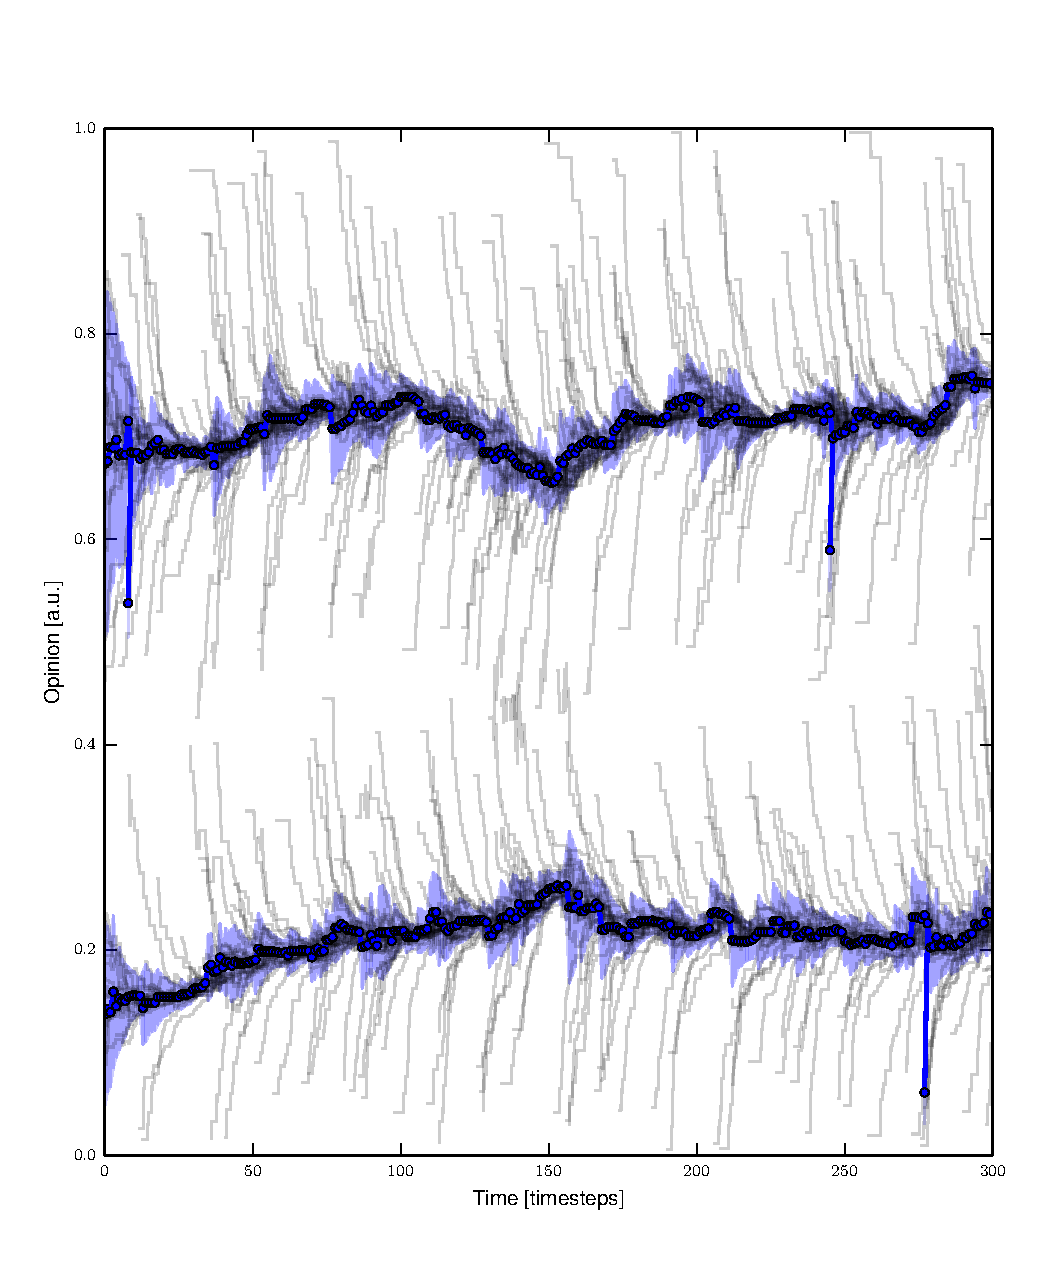
\includegraphics[width=0.45\textwidth]{fig/fiducial.pdf}
    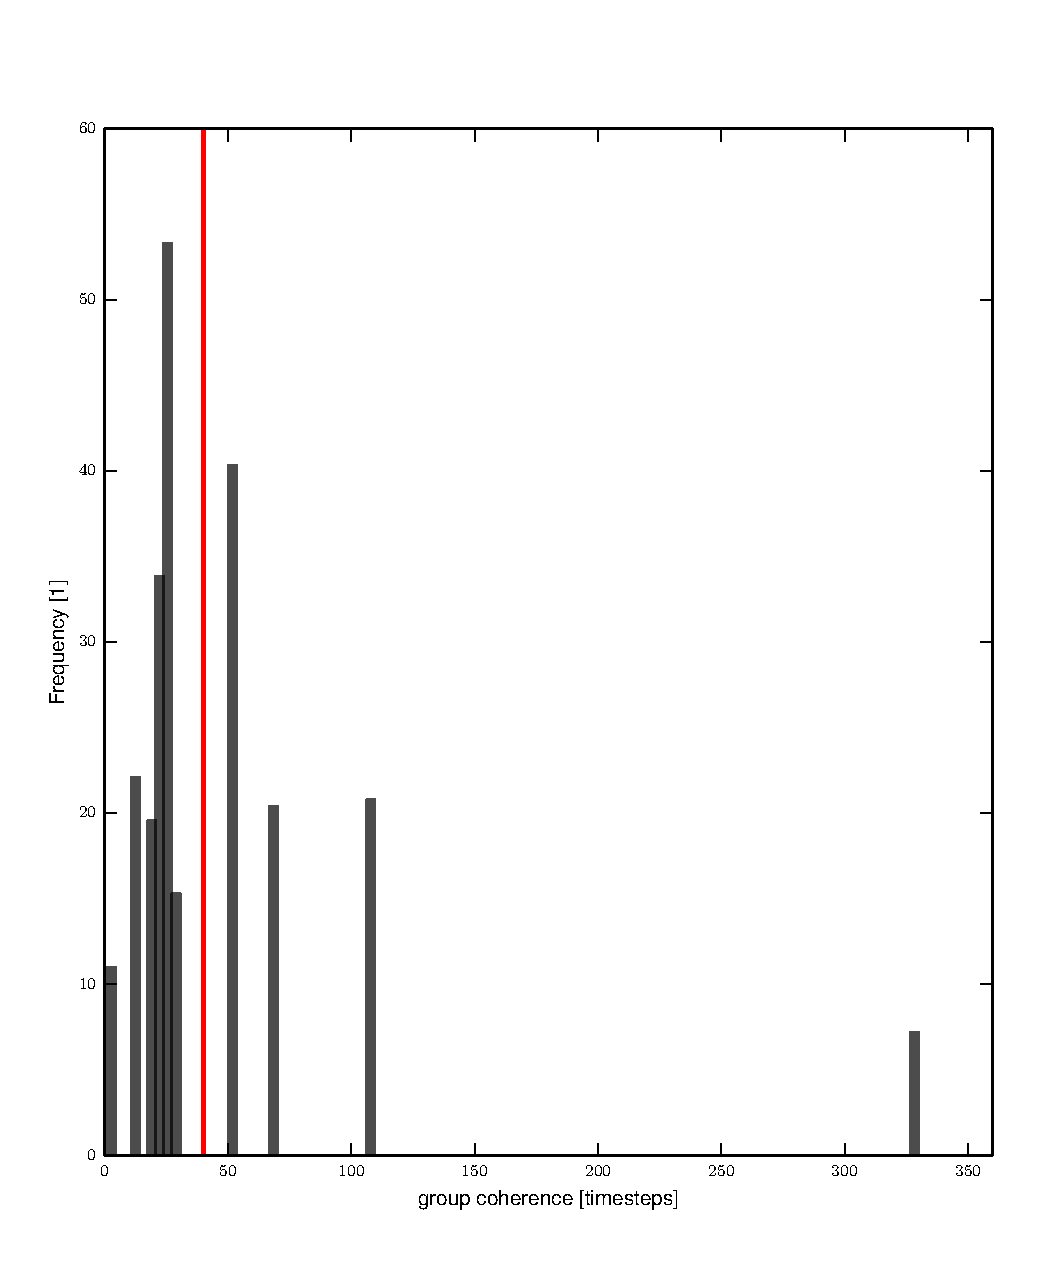
\includegraphics[width=0.45\textwidth]{fig/fiducial_var.pdf}
  \end{center}
  \caption{\label{fig:fiducial} Visualization of the fiducial
    simulation. Gray timelines show the opinion evolution of single
    agents. Blue lines indicate groups, with the standard deviation of
    the contained agents as blue shaded area. See text for definition.
    Right: $\Delta T$ distribution for the groups
    identified in the fiducial simulation fig. \ref{fig:fiducial}. The
    vertical line shows the lifetime of a single agent.}
\end{figure*}

The vertical line depicts the lifetime of a single agent. The
analytically derived approximation for the generation duration lies
close-by, at 45. I get time-spans of the same order of
magnitude, with the split stemming from discreteness effects: If by
chance a group is detected to be disrupted as the number of agents
drops below the critical group detection limit, the maximum timescale 
is shortened. With only two groups over a total of 8 agent
lifetimes, this does not give enough statistics to reject the analytic
hypothesis derived under the assumption of steady state.


\subsection{Array of  Simulations}

I show representations from the parameter sweep: in figures
\ref{fig:20} and \ref{fig:80} the effect of changing the maximum
lifespan, and in figures \ref{fig:01} and \ref{fig:04} the effect of
changing $\varepsilon$.

\begin{figure*}
  \begin{center}
    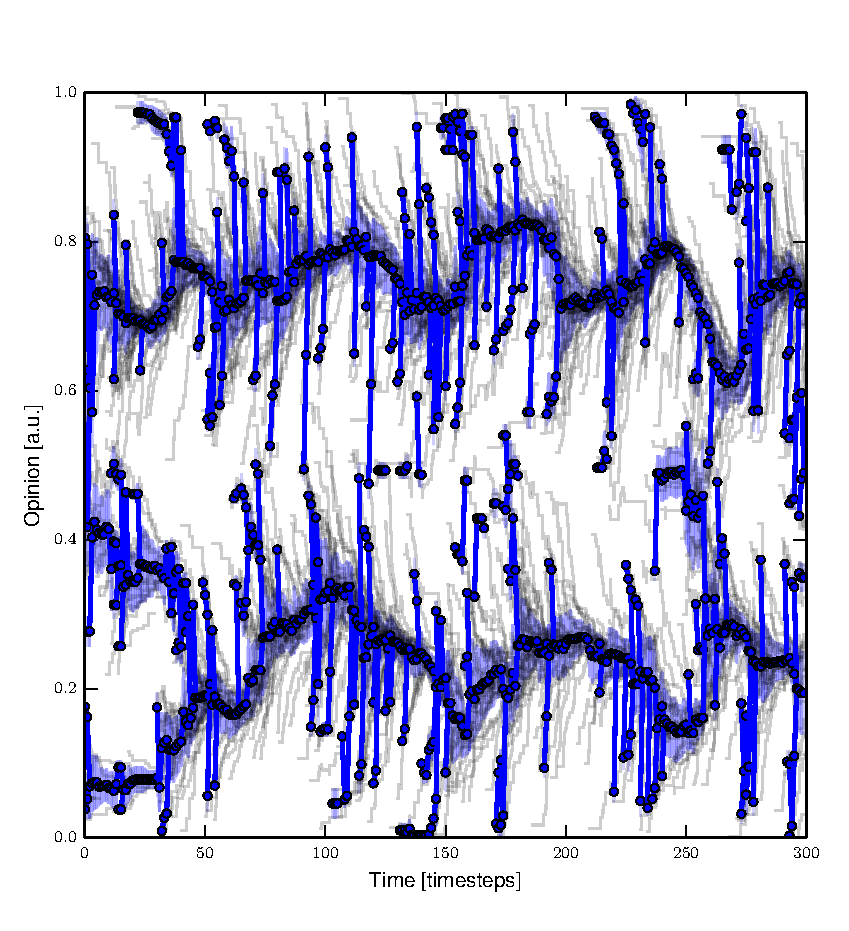
\includegraphics[width=0.3\textwidth]{fig/evol_20.pdf}
    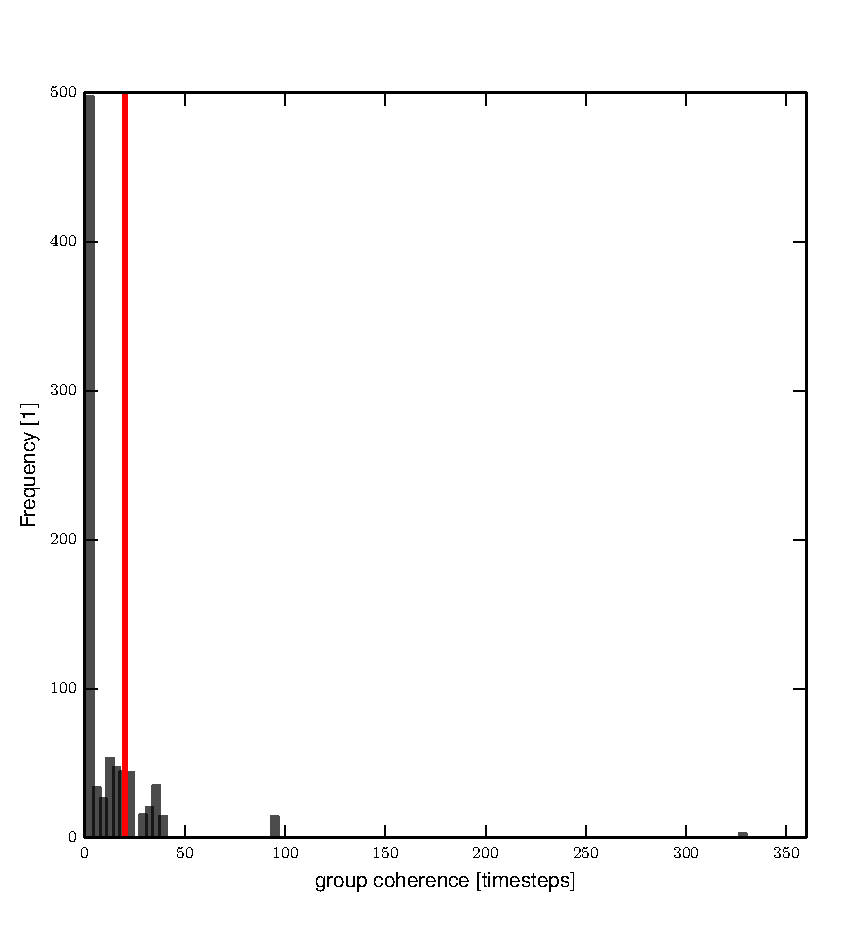
\includegraphics[width=0.3\textwidth]{fig/var_20.pdf}
  \end{center}
  \caption{\label{fig:20}$T_{\rm max}=20$}
\end{figure*}

\begin{figure*}
  \begin{center}
    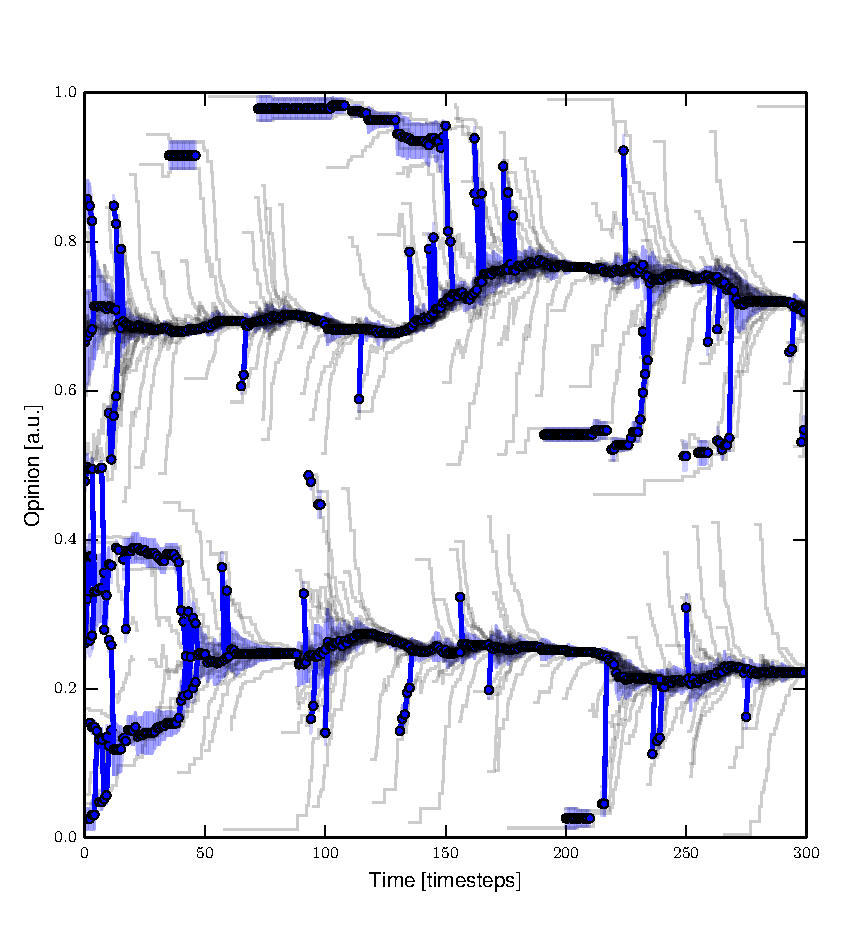
\includegraphics[width=0.3\textwidth]{fig/evol_80.pdf}
    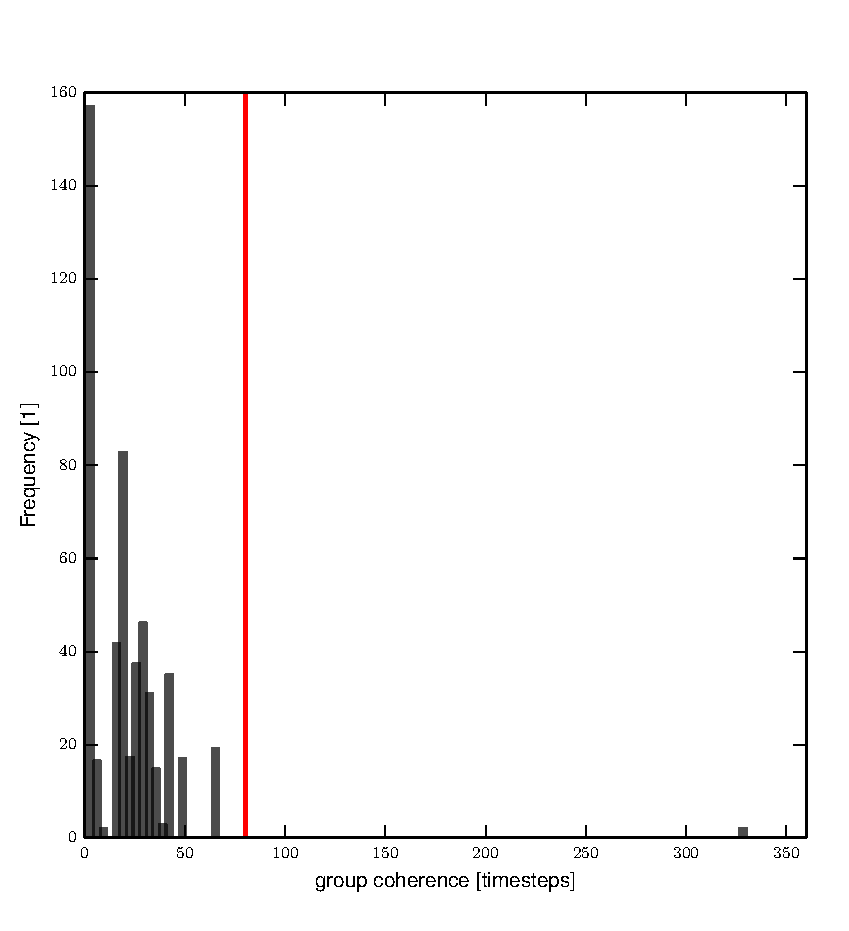
\includegraphics[width=0.3\textwidth]{fig/var_80.pdf}
  \end{center}
  \caption{\label{fig:80}$T_{\rm max}=80$}
\end{figure*}

\begin{figure*}
  \begin{center}
    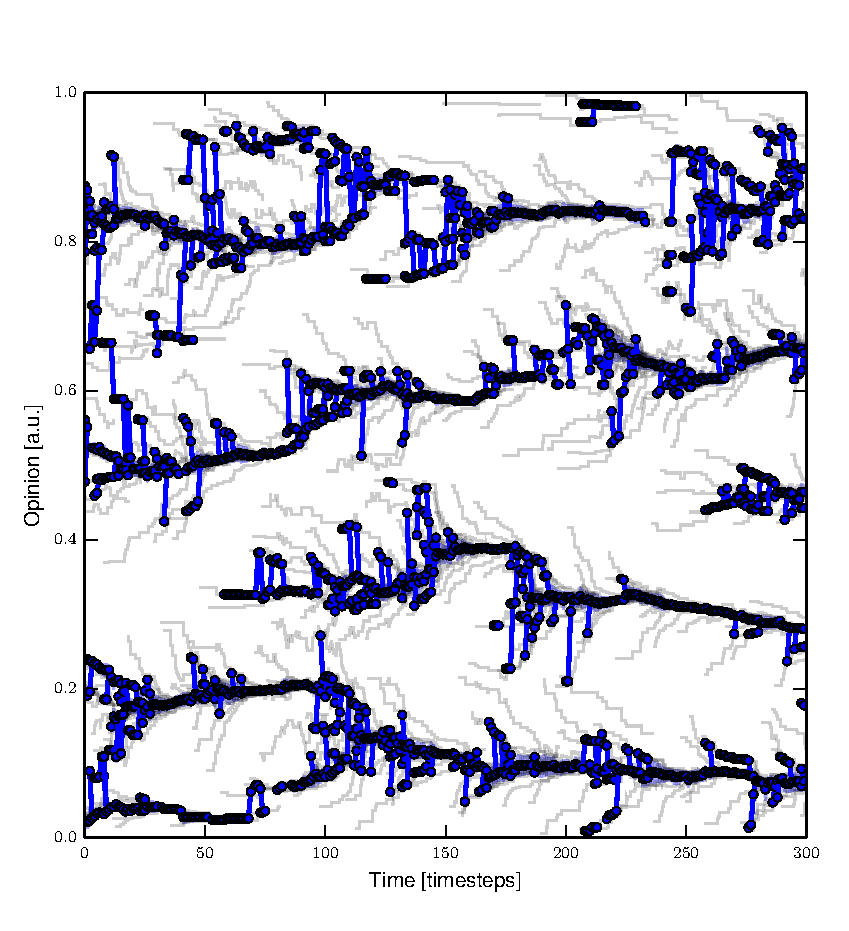
\includegraphics[width=0.3\textwidth]{fig/evol_01.pdf}
    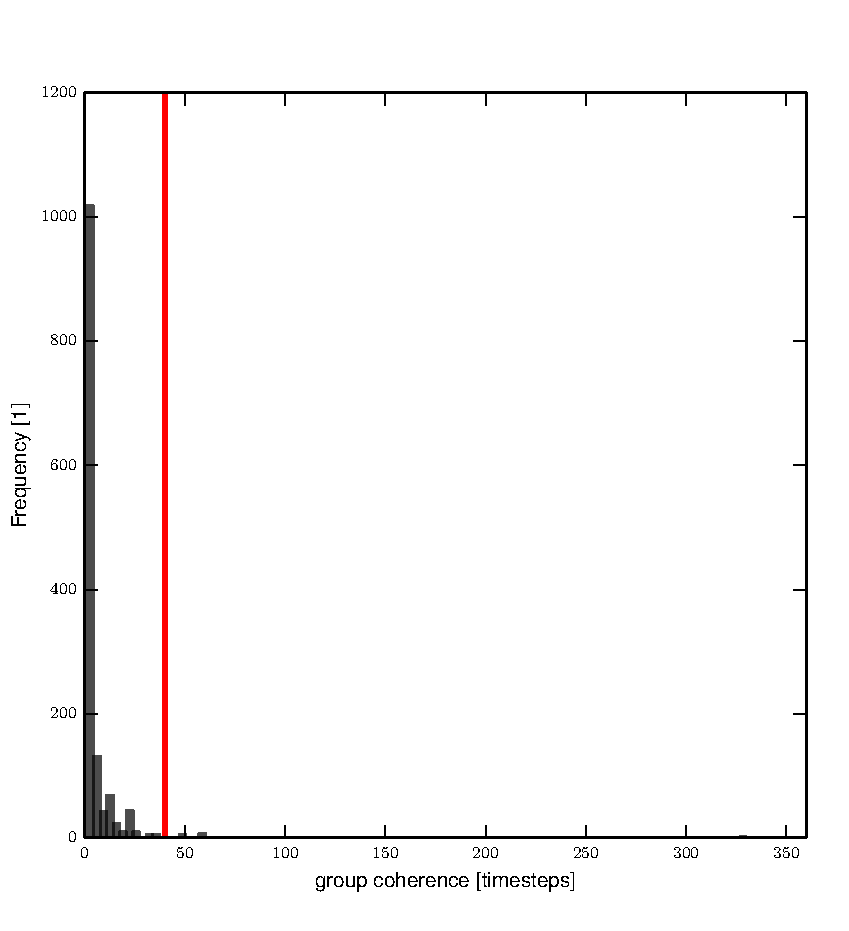
\includegraphics[width=0.3\textwidth]{fig/var_01.pdf}
  \end{center}
  \caption{\label{fig:01}$\varepsilon=0.1$}
\end{figure*}

\begin{figure*}
  \begin{center}
    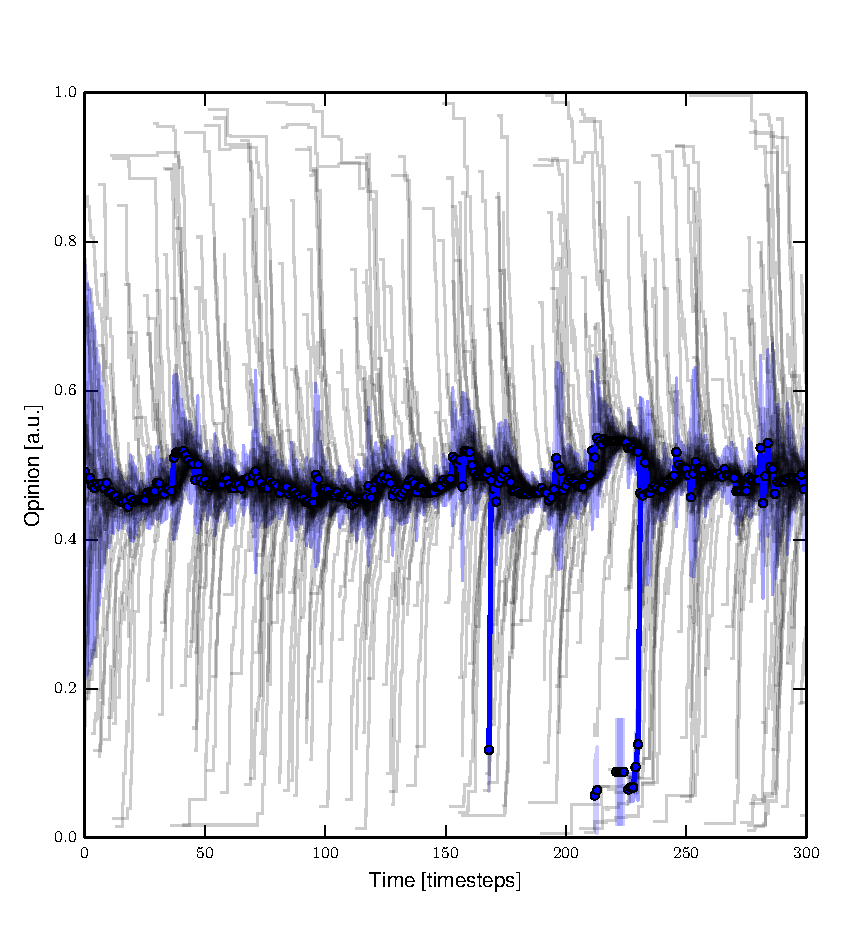
\includegraphics[width=0.3\textwidth]{fig/evol_04.pdf}
    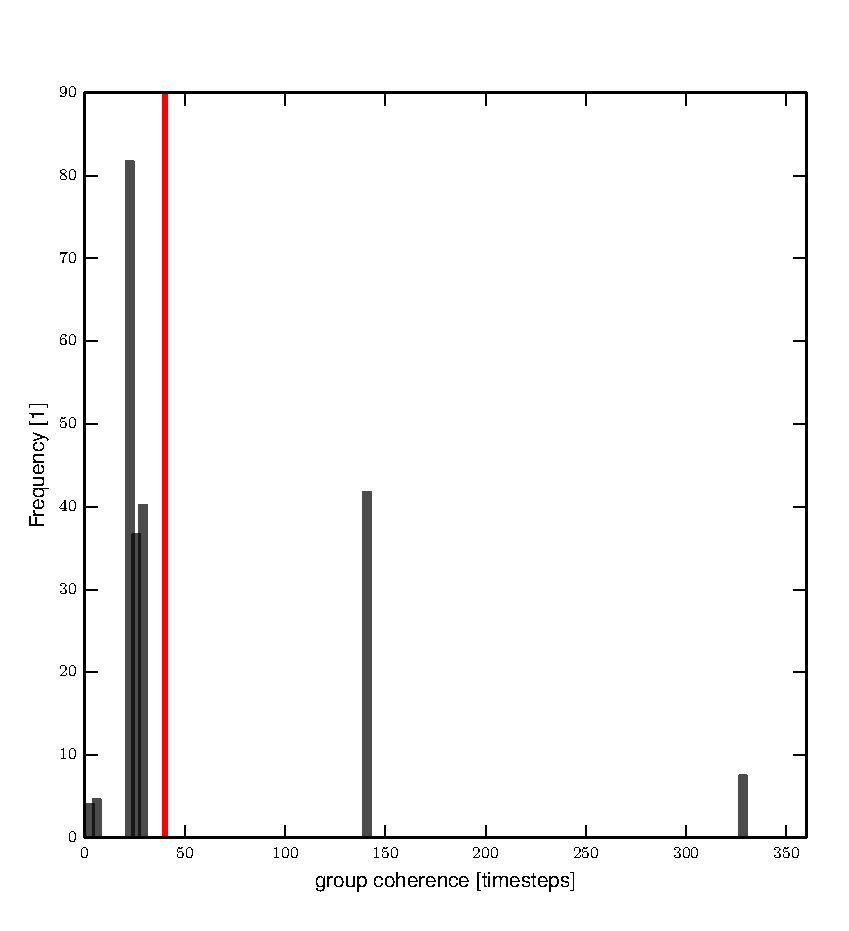
\includegraphics[width=0.3\textwidth]{fig/var_04.pdf}
  \end{center}
  \caption{\label{fig:04}$\varepsilon=0.4$}
\end{figure*}

Reducing the lifetime to $a_{\rm max}=20$ introduces many new
shortlived groups. This comes mainly from the fact that a shorter
lifetime allows more wiggling in the mean opinion of a group. This in
turn comes from a) less old agents to be changed, as they quickly
disappear, and b) a higher frequency of new agents, away from the
consensus. So many in fact, that the group finder algorithm is
identifying clusters of agents away from a consensus. These quickly
evolve back to the nearest group, and thus introduce the peak at small
$\Delta T$. Two opinion groups still evolve for a long time (90
timesteps), but even that one is shorter compared to the fiducial
model, owing to the higher variability of the mean.

Enhancing the lifetime to $a_{\rm max}=80$, on the other hand,
keeps the outliers relatively stable, and shrinks the spread in each
group to smaller values. This then leads to a plethora of consensus
changes as defined above, as a difference of two standard deviations
is reached readily when the standard deviations are small.


For small $\varepsilon=0.1$, one observes more
interruptions in the group classification step, originating from the
discreteness effects as the 50 agents used in the model cannot fully track all possible groups. This means shorter
timescales overall, once from the fact that the old groups disappear
and restart, and secondly from the fact that there are more groups
forming in the regions between the old groups. These groups are highly
susceptible to the influence from their neighbors, and thus quickly
merge.

The other extreme with high $\varepsilon=0.4$ shows more stable
behavior, as almost all agents immediately converge to the central
group, and thus a) keep the mean opinion stable by their high numbers
b) dissolve secondary groups before they become real competitors. The
resulting distribution shows a very high peak at around 3 times the
lifetime, and renders this parameter combination the most stable
configuration under study. Short-term fluctuations happen at a little
under the lifetime, and are comparable to what we previously analyzed
with pen and paper.

\section{Discussion}
\label{sec:discussion}

%TODO{find papers done already}

I include an additional internal parameter in the bounded confidence
model: the age of an agent.

I confirm the hypothesis that opinions evolve significantly away
from the previous consensus value over time if agents
are replaced by new agents with random opinions.

The timescale of significant change is found to be comparable to the lifetime of a single agent.

I derive following consequences for a highly connected society (where distance in
Euclidean space is not important):

\begin{enumerate}
    \item Opinions will not stay in a previously found consensus if
    new people with random opinions appear (either by birth or
    exchange of people by means of transport).
    \item there is only small resilience against quick changes: If people
    do not discuss with people of moderately different opinions (low $\varepsilon$) there is the possibility to
    perform continuous small phase space jumps. If the people are
    long-lived, they will suppress groups of differently-thinking
    people.
    \item Big changes appear to happen on the timescales of the
    order of a lifespan of a single agent. This does {\bf not}
    originate from the fact that old people die all at once. It
    comes from the fact that after a series of consistent opinion
    nudges, the influence from a group of another group with strongly
    differing opinion is visible.
\end{enumerate}


Further investigations should be carried out to include

\begin{enumerate}
    \item spatial distances in the metric to account for the fact that
    consensus does not have to be found globally, but only locally;
    \item stubborn agents, i.e. agents that tend to relax back to their
    initial opinion.
\end{enumerate}

\end{document}
